\subsection{
  Replies to comments received from Thomas Kutter - Aug 20, 2013 }

\begin{enumerate}

  % ........................................................................................................
  \vspace{5 mm}
\item
  {\em
    Page 9, l.371\\
    FGD 1 only, I assume ?
  }\\
  \\
  Correct, this has been updated.

  % ........................................................................................................
  \vspace{5 mm}
\item
  {\em
    Page 10, l.414 and all future occurrences:\\
    single mu-like ring $\rightarrow$ mu-like single ring OR single ring mu-like event  
  }\\
  \\
  Changed to 'single-ring $\mu$-like', as in page 6 of T2K-TN-034. 
  
  % ........................................................................................................
  \vspace{5 mm}
\item
  {\em
    Page 10, l. 426:\\
    - energy scale is 2.3\% in TN 164 $\rightarrow$ please provide and check your reference
  }\\
  \\
  The number 2.4\% comes from Sec.\ 7.2 of T2K-TN-148.
  The reference has been added.
  
  % ........................................................................................................
  \vspace{5 mm}
\item
  {\em
    Page 10, l.437:\\
    How were intranuclear and secondary interaction parameters and uncorrelated cross section parameters split
    into these classifications in the first place ? 
    Now they are being combined into single co-variance matrix. Please add some explanation to motivate this change.
  }\\
  \\
  The uncorrelated cross section errors were given to us by the NIWG.
  Please see TN108 and TN113 for details.

  The SuperK detector error efficiency matrix was given to us by T2KSK.
  Please see TN159 for details.

  The errors on parameters used to generate the FSI+SI matrix were provided by the NIWG.
  Please see TN108 and TN113 for details.
  The form of the FSI+SI matrix was chosen by oscillation analysers
  (both the VaLOR and (as then called) KIT groups)
  during the preparation for the Run 1-3 result,
  so as to have not too many nuisance parameters.
  Please see \url{http://www.t2k.org/asg/fluxmeasure/banffoa091312/numudisapp/view} for details
  of different binning schemes we tried\footnote{
    The 'fine' binning scheme was never completed;
    a covariance matrix for many bins could not be found.
  }.
  The conclusion is that we are not underestimating the error from FSI+SI with the matrix in this 6-bin form.

  The SuperK detector efficiency and FSI+SI matrices have been combined to reduce the number of nuisance parameters
  in the fit, and hence decrease the fit time.
  This is possible, because both the SuperK detector error matrix\footnote{
    TN141 used 3 $E_{reco}$ bins for $\nu_\mu+\bar{\nu_\mu}$ CCQE ring counting efficiency,
    and 1 bin for $\nu_\mu+\bar{\nu_\mu}$ CCQE other efficiencies.
    The 4 'other' and 'ring counting' parameters are combined into 3 parameters,
    giving a 6-parameter SuperK detector efficiency matrix.
  }, and the FSI+SI matrix are binned
  in the same way
  (3 $E_{reco}$ bins for $\nu_\mu+\bar{\nu_\mu}$ CCQE, 1 bin for $\nu_\mu+\bar{\nu_\mu}$ CCNQE,
  1 bin for $\nu_e+\bar{\nu_e}$ CC, 1 bin for NC).
  Fitting the combined matrix is mathematically equivalent to fitting the two matrices independently.
  
  % ........................................................................................................
  \vspace{5 mm}
\item
  {\em
    Page 11, l.442:  (related to Page 10. l. 422 and 424)\\
    was earlier mentioned to now be 6 parameter covariance matrix
    
    It would be good to add a short motivation or expected effect due to this change even in this document.
    As written it is not clear what was actually gained by introducing this.

    Presumably the details will be in TN 159 ?! 
  }\\
  \\
  The 7 parameters referred to in the bullet point are the 1 SuperK energy scale systematic,
  and the 6 parameter SuperK detector efficiency + FSI + SI error matrix.
  The bullet point list \& Tab.\ 1 headings have been updated.

  A sentence has been added to Sec.\ 2.3 to motivate the 7+6 $\rightarrow$ 6 parameter change.

  % ........................................................................................................
  \vspace{5 mm}
\item
  {\em
    Page 14:\\ die $\rightarrow$ due
  }\\
  \\
  Fixed
  
  % ........................................................................................................
  \vspace{5 mm}
\item
  {\em
    Page 14:\\
    $f_{CC\bar{\nu}; t}$  $\rightarrow$ please add reference for the 40\% uncertainty
  }\\
  \\
  This question initiated some email discussion between us and the NIWG convenoors. The summary is:

  \begin{itemize}
  \item The 40\% number came from either
    the most extreme excursions we found with NUANCE variations,
    or from the idea that there were $\sim$20\% discrepancies in neutrino
    CCQE data and theory, and that we weren't sure if those discrepancies would exist, flip sign and/or double, in anti-neutrinos.
  \item This was not included in a technical note.
  \item Since the time 40\% was agreed on (Oct 2012), MiniBooNE and MINERvA have published CCQE results for anti-neutrinos that,
    when compared to neutrino results, make it pretty clear that this 40\% is an overestimate.
    Something closer to 20\% for neutrino and anti-neutrino differences is sufficiently conservative.
  \end{itemize}

  In v3 of the note, we will use the 20\% number.
  
  % ........................................................................................................
  \vspace{5 mm}
\item
  {\em
    Page 18:\\
    why was $\delta_{CP}$ chosen to be zero ?
    
    $\rightarrow$ It would be good to add short explanation for choice of value.
    (e.g. "This is what others do." is not a good explanation.)
  }\\
  \\
  Since $\delta_{CP}$ has not been measured by any experiment, a well motivated choice of value to use
  is impossible.
  The constant-$\Delta\chi^2$ normal hierarchy contours for
  $\delta_{CP} = -\pi/2$, 0, $+\pi/2$, $+\pi$
  is shown
  in Fig.\ \ref{fig:constdchisqcontours_changedcp} of this document.
  It can be seen that changing $\delta_{CP}$ has almost no effect on the contour,
  therefore we feel that our choice of $\delta_{CP} = 0$ was sufficient.

  In v3 of the note, we will fit for $\delta_{CP}$.

  % ........................................................................................................
  \vspace{5 mm}
\item
  {\em
    Page 29:\\
    What causes the center peak to disappear with high statistics ?
    Or rather, what causes the center peak at lower statistics ?
  }\\
  \\
  This is a matter of statistical error.
  In Fig.\ 15, with low statistics, it is possible for the input to be such
  that there is more disappearance than the model allows, hence there
  is a build up of events at the point of maximal disappearance.
  In Fig.\ 16, with high statistics, the error is reduced such that
  the MC toys do not fluctuate enough to exhibit this behaviour.
  
  % ........................................................................................................
  \vspace{5 mm}
\item
  {\em
    Page 32, fig. 27, left most panel second row (and similar in other figures):\\
    Why is this distribution so much narrower ?
  }\\
  \\
  This the parameter is the spectral function.
  In toy experiment creation, it is thrown uniformly between 0 and 1.
  In fits, it is bound between 0 and 1\footnote{
    In v1 of the note, there was a Gaussian constraint applied to this parameter.
    In v3 of the note, we will turn off this constraint.
  }.
  Therefore it is not expected to have the same Gaussian distribution as the other parameters.
  
  % ........................................................................................................
  \vspace{5 mm}
\item
  {\em
    Page 38, Line 671:\\
    remove 4a
  }\\
  \\
  The figure caption was incorrect (Figs.\ 55 \& 56 are Run 1+2+3+4a data fits).
  The caption has been corrected.
  
  % ........................................................................................................
  \vspace{5 mm}
\item
  {\em
    Page 51, Figure 61 $\rightarrow$ Table XX :\\
    This should be table not figure
  }\\
  \\
  Fixed.
  
  % ........................................................................................................
  \vspace{5 mm}
\item
  {\em
    Page 54, fig. 65/66: \\
    "Efficiency holes" seem to be different for different values of $\Delta m^2$ / $\sin^2 \theta$ 
    This makes the plots confusing. Please add better description or unify holes.
  }\\
  \\
  Caption has been clarified.
  
  % ........................................................................................................
  \vspace{5 mm}
\item
  {\em
    Page 54, fig. 66: \\
    How many values of $\Delta m^2$ were considered to generate these plots ?
  }\\
  \\
  Figs.\ 65 \& 66 are an alternative way to represent the information in Fig.\ 64.
  A maximum of 6 values of $\Delta m^2$ were used.
  
  % ........................................................................................................
  \vspace{5 mm}
\item
  {\em
    Page 57, fig. 69:\\
    If I understand correctly const $\Delta \chi^2$ has $\delta_{CP}=0$ and whereas for FC method delta is randomized between $-\pi$ and $+\pi$.
    Please clarify whether the 3 flavor oscillation formula approximation from footnote on p.29 was used or whether delta dependent
    terms have been included. I assume the latter but please confirm.

    How do the const. $\Delta \chi^2$ contours change as function of delta ? 
    And why was delta =0 chosen ?  
  }\\
  \\
  All terms (including matter effects) are included in the oscillation probabilities.
  The purpose of the footnote is to show where the point of maximum disappearance approximately is,
  and it's dependce on the value of $\sin^2\theta_{13}$.

  Since $\delta_{CP}$ has not been measured by any experiment, a well motivated choice of value to use
  is impossible.
  The constant-$\Delta\chi^2$ normal hierarchy contours for
  $\delta_{CP} = -\pi/2$, 0, $+\pi/2$, $+\pi$
  is shown
  in Fig.\ \ref{fig:constdchisqcontours_changedcp} of this document.
  It can be seen that changing $\delta_{CP}$ has almost no effect on the contour,
  therefore we feel that our choice of $\delta_{CP} = 0$ is sufficient.

  In v3 of the note, we will fit for $\delta_{CP}$.

  
  % ........................................................................................................
  \vspace{5 mm}
\item
  {\em
    Page 57, fig. 70:\\
    It would be better to compare run 1-3 results and run 1-4 results more directly by using same treatment of octant.
  }\\
  \\
  We feel the best way to present comparisons is in terms of $\sin^2\theta_{23}$, and this plot
  has been added in v2 of the note.
  
  Fig.\ \ref{fig:contours_sinsq2theta_method} of this document shows the run 1-4a normal hierarchy contour converted into $\sin^2(2\theta_{23})$ in 3 ways:
  \begin{itemize}
  \item profiling over the octant, as in Fig.\ 70;
  \item assuming the first octant;
  \item assuming the second octant.
  \end{itemize}
  It can be seen that profiling is equivalent to the second octant assumption.

  Fig.\ \ref{fig:contours_sinsq2theta_external} of this document is a version of Fig.\ 70 with the two octant assumptions
  for the constant-$\Delta\chi^2$ method only.

  \begin{figure*}[htb]
    \center
    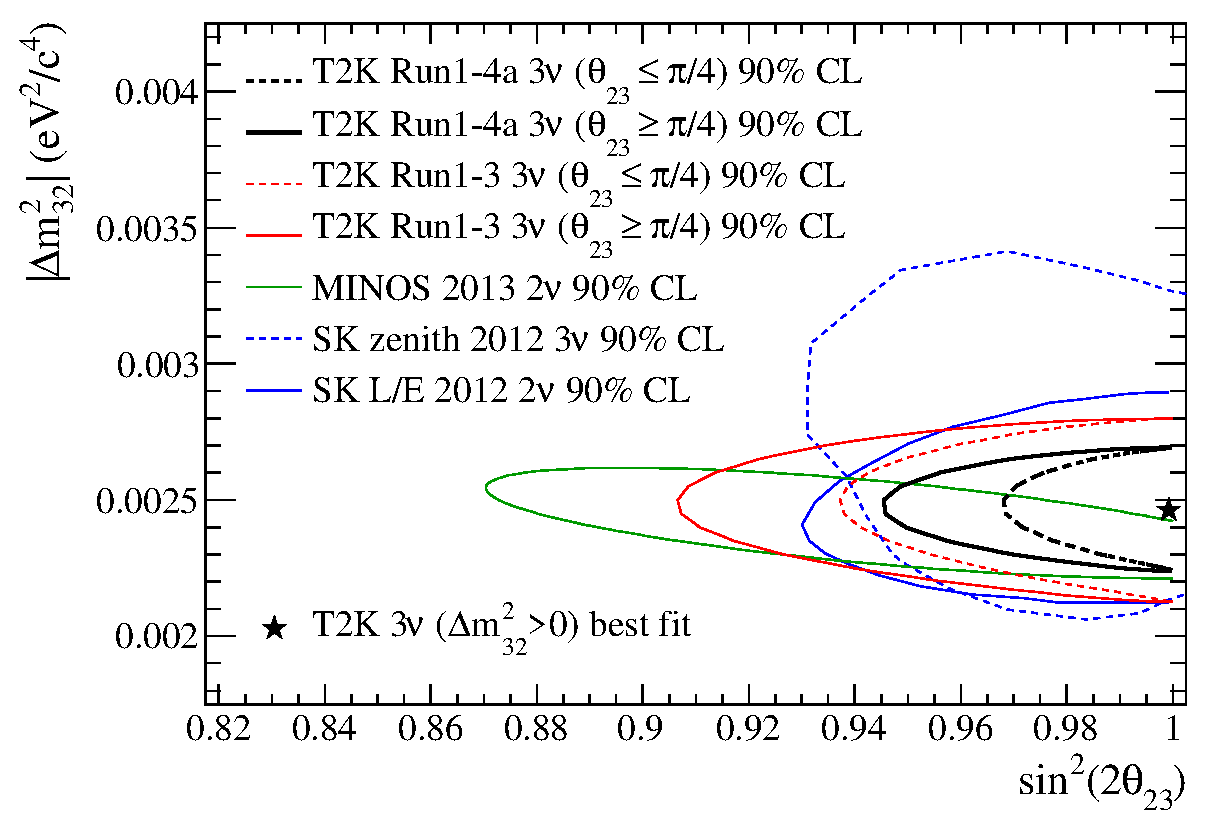
\includegraphics[width=30pc]{./images/contour_compare_constdchisqoctants_external_sinsq2theta23}
    \caption {
      Comparison between 90\% CL allowed regions 
      from MINOS, SuperK atmospherics, T2K Run 1+2+3,
      and the 90\% CL regions obtained from the VaLOR fit to the Run 1+2+3+4a dataset.
      Contours are obtained using the constant-$\Delta\chi^2$ method, and contours for both octant assumptions are shown.
      The normal mass hierarchy is assumed for all results.
    }
    \label{fig:contours_sinsq2theta_external}
  \end{figure*}


  %........................................................................................................

\end{enumerate}






 


 


 


 


 


 

 

